\documentclass[11pt, a4paper]{article}
\setlength{\oddsidemargin}{0.5cm}
\setlength{\evensidemargin}{0.5cm}
\setlength{\topmargin}{-1.6cm}
\setlength{\leftmargin}{0.5cm}
\setlength{\rightmargin}{0.5cm}
\setlength{\textheight}{24.00cm} 
\setlength{\textwidth}{15.00cm}
\parindent 0pt
\parskip 5pt
\pagestyle{plain}

\title{Research Proposal}
\author{}
\date{}

\newcommand{\namelistlabel}[1]{\mbox{#1}\hfil}
\newenvironment{namelist}[1]{%1
\begin{list}{}
    {
        \let\makelabel\namelistlabel
        \settowidth{\labelwidth}{#1}
        \setlength{\leftmargin}{1.1\labelwidth}
    }
  }{%1
\end{list}}

\usepackage{graphicx}
\graphicspath{ {../figs/} }
\usepackage{hyperref}

\begin{document}
\maketitle

\begin{namelist}{xxxxxxxxxxxx}
\item[{\bf Title:}]
	Black Box System Model Learning and Verification.
\item[{\bf Author:}]
	Johnathan DiMatteo
\item[{\bf Supervisor:}]
	Sebastian Fischmeister
\item[{\bf Degree:}]
	MMath
\end{namelist}

\section*{Motivation} 
% In this section you should give some background to your
% research area. What is the problem you are tackling, and why is it
% worthwhile solving? Who has already done some work in this area,
% and what have they achieved?

%What is IoT?
%The recent explosion of the Internet of Things (IoT) puts numerous embedded devices at the hands of governments, businesses, and consumers.
%There will be as many as 50 billion IoT devices around the world by 2020 \cite{iotcisco}.
%Their low cost has caused manufacturers to produce and sell them without sufficient security or safety features \cite{iotsec}.
%If action is not taken, vulnerabilities in IoT devices can lead to harm both economically and otherwise.

To enforce security and safety in devices, models must be validated.
Validating a model ensures anomalous states and transitions are corrected to avoid security vulnerabilities.
One proposed method to do this is a process of reverse engineering the system, called \textit{Model Learning}.
Model learning aims to construct blackbox state diagram models of software and hardware systems by providing inputs and observing outputs \cite{modellearning}.
This has been a fundamental research problem studied for decades, but two recent advancements have allowed us to propose a new method.
First, \textit{side channel analysis} has allowed us to study a system's response without the need to open the so called ``black box''.
By treating a device as a black box system, one can monitor the power consumption to provide a non-intrusive approach \cite{seb}.
Traditional modelling tools can introduce timing errors and other anomalies. 
The downside to this approach is the complexity of the response (ie. it is now a time series signal instead of a binary output).
But \textit{machine learning} has opened new data driven approaches for dealing with time series modeling, allowing us to cluster signals to states.
Useful in many areas.
One possible application could be during Hardware in the Loop (HIL) testing to identify unwanted or undocumented functionality.
A well trained model can identify flaws in the design of IoT devices to enforce security and safety.

\section*{Problem Statement} 
%Now state explicitly the hypothesis you aim to
%test. Make references to the items listed in the Reference section
%that back up your arguments for why this is a reasonable
%hypothesis to test, for example the work of Knuth~\cite{knuth}.
%Explain what you expect will be accomplished by undertaking this
%particular project.  Moreover, is it likely to have any other
%applications?

\begin{enumerate}
    \item \textbf{Change Detector}: Given a black box system, determine internal state changes in response to inputs in order to learn the system's behaviour.
    \item \textbf{Input Generator}: Given inputs and knowledge of previous state changes, what should be the next query to the system?
\end{enumerate}

\section*{System}

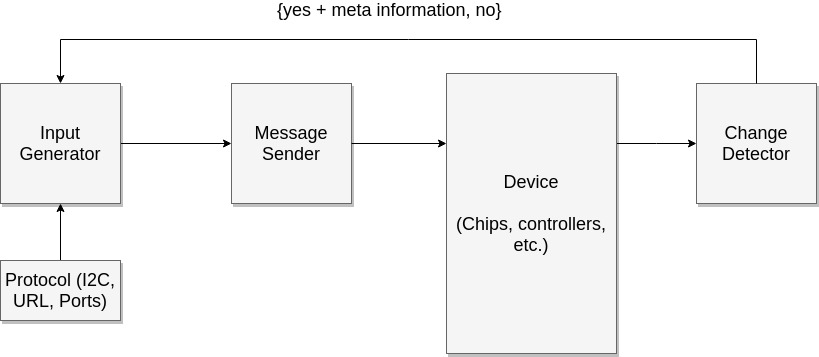
\includegraphics[scale=0.5]{Fuzzer.png}

\subsection*{State Detector}
The State Detector needs to be able to determine what state the system is in given a response.
There are several ways to do this.
distance based: measure of how much the signal moved
dtw: define a threshold. larger difference = more confident.

clustering algorithms: do they require us to input no. of states? online learning? confidence?
options: dbscan, k means (dont know many clusters though)
DBSCAN is good, no states required, identifies noise. BUT we have to recalculate with all data points, every time (BUT only do DTW once, ie. 
receive batch of responses, cluster, return yes + msg that triggered it, or no or maybe or more than one + msgs.

Bayesian approach: DETERMINE WHICH CLUSTER OR MAKE A NEW ONE. can eliminate noise manually or just accept it.
for each state, build an expected signal. that way we save out on memory. 
if the expected signal has an extremely high standard deviation ... it might be time to make a new cluster
but we need some way of matching up signals (apparently you can align them using cross correlation, or custom change detection ie. significant change)
compute dtw distance to each expected state signal. (or cluster)
return (current state) or (new state, msg that triggered it)
 
%\begin{enumerate}
%    \item receive signals
%    \item align signals using cross correlation
%    \item sample from expected signals (each representing a state) and add those to the group
%    \item cluster the group using DBSCAN algorithm
%    \item iterate through labels: if a label is in the same group as an expected signal, add it to the signal, update expected signal and state data. Else create a new state.
%\end{enumerate}
%
%or \\

\begin{enumerate}
    \item receive a response
    \item calculate dtw to every expected state response
    \item if within $\epsilon$ of one state, add it to the closest state. else if its within $\epsilon$ of two or more clusters, try joining them together. else not within $\epsilon$ of any: create a new state (parameter $\epsilon$: HOW CAN WE TUNE ITif 
    \item align and re-compute expected state response
    \item return (state (string), change detected (bool), distance to closest state?).
\end{enumerate}

question: what should $\epsilon$ be? how can we tune it?\\
question: how can we get confidence levels of being in a state?\\

parameters: $\epsilon$
data: expected signals per state, number of signals per state, standard deviation per state

returns: (state(s), confidence) indicating the state change(s) and the message(s) that triggered it.

\subsection*{Input Generator}

needs to know current state.
enumerate through all possibilities at current state (ie. for I2C, write to each bit of one register, send all at once... )
problem: what if we change states and then change again quickly? it would appear as noise. so we need to be careful with noise.
Change Detector returns all states it has observed and the trigger messages.
Log states and trigger messages.
If last state is a new state, repeat. 
Elif (we have seen it before): pick a state we have not been to before.
Else all states have been reached: end.
note: need to verify that all write operations are the same and change with state. have only done so with reads.

\begin{enumerate}
    \item receive state
    \item try to change the state: send a bunch of messages while modifying one bit at a time depending on protocol (character for URL, bit for NMAP packets).
\end{enumerate}

question: how can we determine which msg to send given a state? see \href{https://en.wikipedia.org/wiki/Active_learning_(machine_learning)}{Active Learning}, in particular, uncertainity sampling.
To do uncertainity sampling we need to know the probability of being in a state (the confidence) to be returned by the state detector. \\

parameters: protocol specification (json?)
returns: message to send

notes:\\
L star algorithm: can't because we don't have an oracle that can give us a counterexample, unless we search and depend on our clustering algorithm?
also we dont have a way to deal with non-determinism\\
randomization is going to be important since we are exploring\\
There are ways to have error: given state A if we expect to go to B from experience but we go to a new state C, thats an error\\
perhaps genetic algorithms? first we explore a little to build a model then we train? 
ie. which messages are trigger messages? start with a random selection,
keep ones that trigger a state change, 
refresh new ones ? \\

\section*{Message Sender}
Determined by protocol.
Focus on I2C for now.

\section*{Additional Modules or Functionality}
method to convert states and transitions to mealy machine.\\
message sender (already implemented for I2C)
focus will be on I2C since system is already in place.\\
function to plot expected signals ie. what do they look like\\

Data model: json? file that stores all states and state transitions.\\

\section*{Applications}
model Verification\\
model security: can alert users if system is operating outside expected behaviour per state.\\

\end{document}


